\begin{frame}
  \frametitle{Plan du cours}
\tableofcontents

\end{frame}

\section{Cluster ou Partitionnement de données}
\subsection{Définition}

\begin{frame}
  \frametitle{Le Clustering une discipline de Machine learning}

 \begin{figure}
  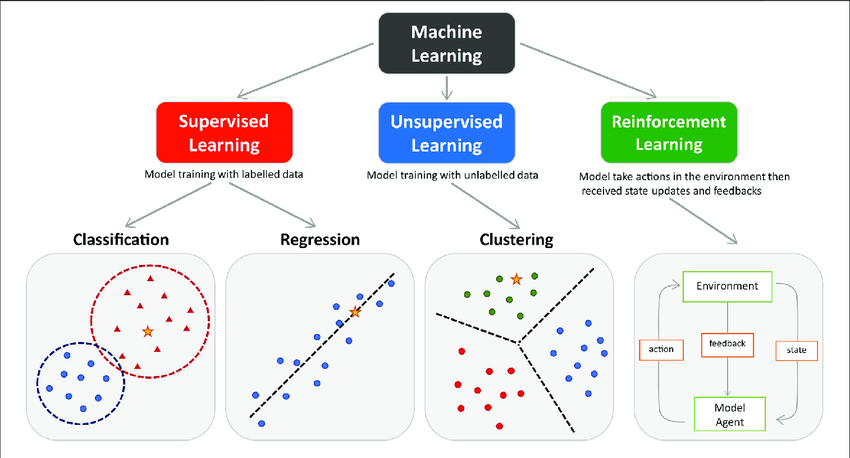
\includegraphics[width=10cm]{images/The-main-types-of-machine-learning-Main-approaches-include-classification-and.png}
  \caption{\url{https://www.frontiersin.org/journals/pharmacology/articles/10.3389/fphar.2021.720694/full}, \cite{10.3389/fphar.2021.720694}}
  \end{figure}
\end{frame}

\begin{frame}
  \frametitle{Définition\footnote{\url{https://fr.wikipedia.org/wiki/Cluster},Wikipédia} }
   \begin{description}
  \item [Général] \textit{Groupement d'un petit nombre d'objets.}
  \item [Linguistique] \textit{groupe consonantique, il correspond à une succession d'au moins deux consonnes dans un mot. Par exemple, dans fraise ou tigre. On retrouve parfois des clusters plus complexes. }
  \item [Informatique 1]\textit{ grappe de serveurs sur un réseau}
  \item [Informatique 2] \textit{une base de données distribuée dans des grappes de serveurs - MySQL Cluster}
  \item [Informatique 3] \textit{« Data clustering » désigne l'analyse de \textbf{partitionnement de données}.}
  \end{description}


\end{frame}

\begin{frame}
  \frametitle{Le partitionnement de données\footnote{\url{https://dataanalyticspost.com/Lexique/clustering/}}}


 \begin{itemize}
  \item \ding{107} Méthode de classification non supervisée, 
  \item \ding{107} algorithmes d’apprentissage 
  \item \ding{107} regrouper des données non étiquetées selon des propriétés similaires
  \item \ding{107} Isoler des schémas/familles
  
  
 \end{itemize}
 


\end{frame}


\subsection{Usages}
\begin{frame}
  \frametitle{ à quoi ça sert ?}
 \ding{107} En machine learning
  \begin{itemize}
  \item \ding{220} préparer l’application d’algorithmes d’apprentissage supervisé \ding{222} \textbf{KNN}.\\
\item \ding{220} utilisé lorsqu’il est coûteux d’étiqueter le données.
\end{itemize}

 \begin{figure}
  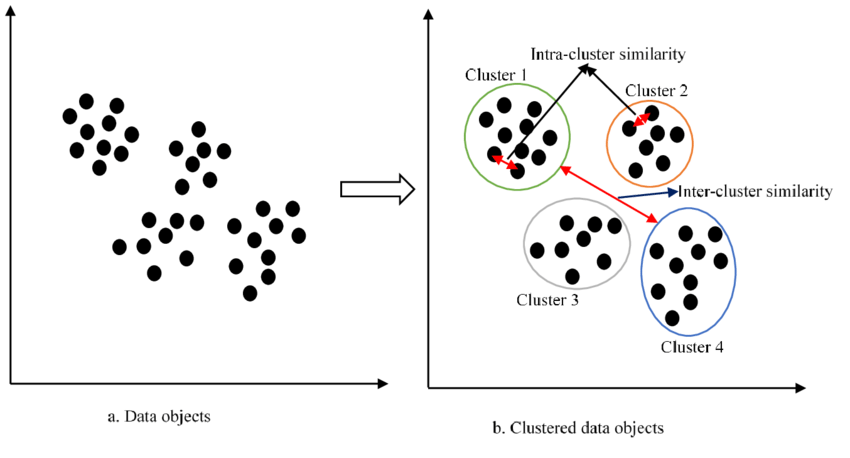
\includegraphics[width=7cm]{images/Clustering-example-with-intra-and-inter-clustering-illustrations.png}
  \caption{\url{https://www.researchgate.net/figure/Clustering-example-with-intra-and-inter-clustering-illustrations_fig1_344590665}, \cite{10.1007/s00521-020-05395-4}}
  \end{figure}
  
\end{frame}

\begin{frame}
  \frametitle{à quoi ça sert ?}
 \ding{107} En TAL
 \begin{itemize}
  \item \ding{220} Regrouper des textes
  \item \ding{220} Regrouper des mots 
  \end{itemize}
  
  \ding{229} selon :
  \begin{itemize}
  \item \ding{220} des caractéristiques linguistique commune (par. ex : quantité de verbes, noms, verbes etc.)
  \item \ding{220} leur sens \ding{222} partitionnement sémantique
  \end{itemize}

\end{frame}

\begin{frame}
  \frametitle{Logique du plus proche voisin}
  Algorithme du plus proche voisin, \textit{K-nearest neighbors} (KNN ou K-NN)\footnote{\url{https://fr.wikipedia.org/wiki/M\%C3\%A9thode_des_k_plus_proches_voisins}},\footnote{\url{https://mrmint.fr/introduction-k-nearest-neighbors}}
  \begin{itemize}
  \item \ding{220} méthode d’apprentissage supervisé,
  \item \ding{220} utilisé pour la classification et la régression,
  \item \ding{220} pas de phase d’apprentissage \ding{222} Lazy Learning. L'algo. généralise directement à partir du jeu de données.
  \item \ding{220} Observe la similarité des K voisins les plus proches. K = nombre entier
  \end{itemize}
   \ding{229} \textit{"dis moi qui sont tes voisins, je te dirais qui tu es…"}
\end{frame}

\subsection{Limites}
\begin{frame}
  \frametitle{Les limites du partitionnement de données}

\ding{107} Pour les mêmes données, peuvent être utilisées :

\begin{itemize}
  \item \ding{220} différentes métriques,
  \item \ding{220} différentes représentations des données 
 \end{itemize}

\ding{220} il peut y avoir des variations/différents regroupements dans les clusters en sortie   

\ding{107} Choisir la méthode dont vous partitionnez les données en considérant :

 \begin{itemize}
  \item \ding{107} les résultats attendus,
  \item \ding{107} l’utilisation prévue des données
 \end{itemize}
\end{frame}

\subsection{Méthodes et Algorithmes}
\begin{frame}
  \frametitle{Le clustering en TAL : quelles méthodes}
\ding{107} Méthodes et Algorithmes :
  \begin{itemize}
  \item \ding{220} hiérarchique : dendogrames
  \item \ding{220} centroïde : K-mean, Affinity Propagation
  \item \ding{220} densité : \textit{« density-based spatial clustering of applications with noise »} - DBSCAN
  \item \ding{220} maximisation de l’espérance (EM) : outils mathématiques probabilistes (Loi Gausse - \textit{Gaussian Mixture model}\footnote{\url{https://dridk.me/expectation-maximisation.html}})
  \end{itemize}
\end{frame}

\begin{frame}
  \frametitle{Regroupement hiérarchique}
  
 \ding{220} Méthodes de classification, « ascendantes » et « descendantes »
\begin{description}
\item  [descendante hiérarchique] 
\begin{itemize}
\item \ding{220} solution générale vers une autre plus spécifique.
\item \ding{220} une seule classe contenant la totalité puis se divisent à chaque étape selon un critère jusqu’à l’obtention d’un ensemble de classes différentes.
\end{itemize}
\end{description} 
\end{frame}

\begin{frame}
  \frametitle{Regroupement hiérarchique}
\ding{220} Méthodes de classification, « ascendantes » et « descendantes »  
 \begin{description} 
\item [ascendantes]
\begin{itemize}
\item \ding{220} tous les individus sont seuls dans une classe \ding{221} en classes de plus en plus grandes. 
\item \ding{220} répartir les individus dans un certain nombre de classes.
\item \ding{220} usage de similarités/distances.
\end{itemize}
\end{description} 
 
\begin{figure}
  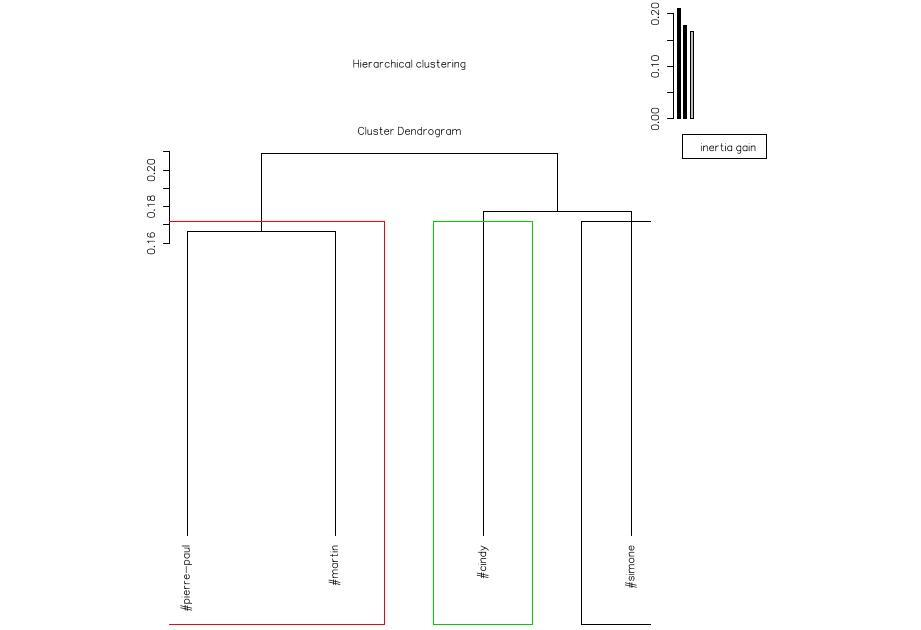
\includegraphics[width=6cm]{images/dendrogramme_img-3.jpg}
  \caption{\url{https://journals.openedition.org/revuehn/3683}, \cite{Melancon2023}}
  \end{figure}

  
\end{frame}

\begin{frame}
  \frametitle{Centroïde}
 \ding{107} k-moyennes. 
  
\begin{itemize}
 \item \ding{192} choix de départ : k, le nombre de classes voulues.k points au hasard parmi les n individus.
  \item \ding{193} k points = k classes;  
  \begin{itemize}
  \item \ding{220} On associe ensuite chacun des n-k points restants à la « classe-point » qui lui est la plus proche.
  \item \ding{220} chaque classe est caractérisée par la moyenne des valeurs de chacun de ses individus. On a k moyennes pour k classes.
  
  \end{itemize}
  \item \ding{194} La deuxième étape consiste à évaluer la distance de chaque individu à chacune des k moyennes.   
  \begin{itemize}
  		\item \ding{220} Certains individus peuvent ici changer de classe.
  		\item \ding{220} A la fin de cette étape, on actualise les k moyennes.
  		\item \ding{220} Et on réitère les étapes, jusqu’à ce qu’il y ait convergence pour obtenir nos k clusters finaux. 
  \end{itemize}
  % \item \ding{194}
  \end{itemize}
 \end{frame}
 
 \begin{frame}
  \frametitle{Centroïde}
\ding{107}Limites
\begin{itemize}
  		\item \ding{220} Les classes finales dépendent beaucoup des k individus choisis pour l’initialisation. 
  		\item \ding{220} La moyenne tient parfois trop compte des valeurs aberrantes.
  \end{itemize}


\ding{220} Certains algorithmes k-means font la somme des distances des individus d'une même classe pour minimiser la variance intra-classe.\\


\ding{220} D’autres représentants que le centroïde (la moyenne) \ding{222} le médoïde l'individu le plus central du groupe.

  
\end{frame}

\begin{frame}
  \frametitle{Densité}
 Zones de densité relativement élevées, zones où beaucoup de points sont proches par rapport à d’autres.

DBSCAN : Algorithme forme des classes d’individus \& repère les valeurs hors du commun/bruit. 

Entrées :
\begin{itemize}
\item \ding{220} la distance maximale qui peut définir deux individus comme voisins,
\item \ding{220} le nombre minimal d’individus nécessaires pour former un groupe.
\end{itemize}

En sortie sont stockés :
\begin{itemize}
\item \ding{220} les clusters successifs
\item \ding{220} les individus visités au fur et à mesure.
\end{itemize}

\end{frame}

\begin{frame}
  \frametitle{A densité}
\ding{100} Etape 1 :\\
\ding{81} choisir un point parmi ceux disponibles. \\
\ding{81} Les distances permettent de définir les plus proches voisins. 


\textcolor{red}{\ding{53}} Si le nombre minimal de point n'est pas atteint, point initial == bruit. \\
\ding{229}On stocke le point dans les individus visités.\\

\textcolor{green}{\ding{51}} Si le nombre minimal de point est dépassé, point initial == initialisation d'un cluster.

 \ding{220}On étudie chaque point à partir de son voisinage initial. \\
\end{frame}

\begin{frame}
  \frametitle{A densité}
\ding{100} Etape 2 :\\

\ding{220} Vérification que le voisinage de chaque point comporte plus d'éléments que le minimum requis \\
\ding{220} on étend le voisinage initial en le réunissant avec le voisinage du point visité.\\

\ding{220} Puis on ajoute ce point dans le cluster. \\
\end{frame}

\begin{frame}
  \frametitle{A densité}
\ding{100} Etape 3 : \\

\ding{220} L'opération est itérée tant que tous les individus n'ont pas été observés \\
\ding{220} Lorsque tous les points du voisinage ont été testés, ceux retenus == stockage individus dans cluster \\
\ding{220} A la fin on obtient :
\begin{itemize}
\item \ding{220} liste de groupes d’individus 
\item \ding{220} les individus correspondant à du bruit, ils ne sont dans aucun cluster. 
\end{itemize}
\end{frame}

\begin{frame}
  \frametitle{Pour aller plus loin}

\begin{figure}
  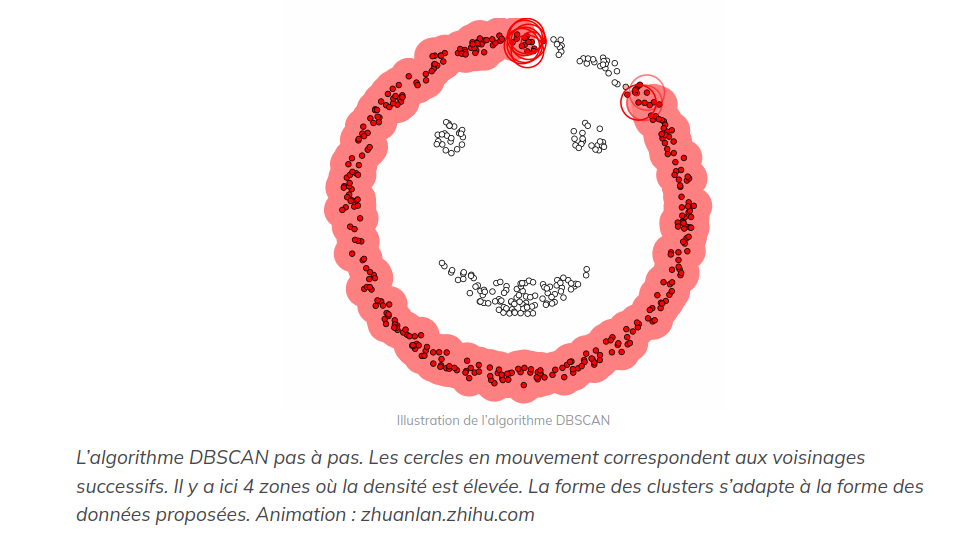
\includegraphics[width=6cm]{images/cluster_densite.png}
  \caption{\url{https://larevueia.fr/clustering-les-3-methodes-a-connaitre/}.}
  \end{figure}
  
Il existe de nombreux algorithmes et méthodes pour partionner les données :
\url{http://www.metz.supelec.fr/metz/personnel/vialle/course/BigData-2A-CS/slides-pdf/13-MachineLearning-Clustering-2spp.pdf}

  
\end{frame}




